\documentclass[11pt]{amsart}
\usepackage{geometry}                % See geometry.pdf to learn the layout options. There are lots.
\geometry{letterpaper}                   % ... or a4paper or a5paper or ... 
%\geometry{landscape}                % Activate for for rotated page geometry
%\usepackage[parfill]{parskip}    % Activate to begin paragraphs with an empty line rather than an indent
\usepackage{graphicx}
\usepackage{subfigure}
\usepackage{amssymb}
\usepackage{epstopdf}
\DeclareGraphicsRule{.tif}{png}{.png}{`convert #1 `dirname #1`/`basename #1 .tif`.png}

\title{Tiling with Right Triominos}
\author{Math 300}
%\date{}                                           % Activate to display a given date or no date

\begin{document}
\maketitle
%\section{x}
%\subsection{}




To {\bf tile} a shape is to completely cover it with smaller shapes so that there is no overhang for the smaller shapes on top of the larger shape.  \vspace{.5cm}

You are allowed to rotate the shapes as if you were playing tetris.  This is a {\bf right triomino}.  It is constructed from three unit ($1 \times 1$) squares.

\begin{figure}[h]
  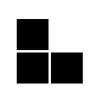
\includegraphics[scale=.60]{triomino}
   \caption{Right triomino}
\end{figure}


Consider an $n \times n$ board.  That is a square board with width $n$ units and length $n$ units.  For example this is a $6 \times 6$ board.

\begin{figure}[h]
  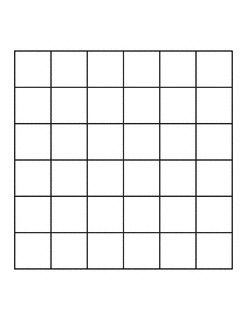
\includegraphics[scale=.50]{66board}
   \caption{6 $\times$ 6 Board}
\end{figure}  

This worksheet is asking questions about tiling a $n \times n$ board with right triominos.

\clearpage

 {\bf Question 1} For $n=1$, 2, 3, 4, and 5, can you completely tile a $n \times n$ checkerboard with a right triomino pieces? You will have an answer for each $n$.\vfill

{\bf Question 2} For $n=1$, 2, 3, 4, and 5, can you completely tile a $n \times n$ checkerboard with a right triomino pieces if one $1 \times 1$ square of the board is removed?  That is if, you do not have to cover exactly one of the tiles, can you then tile the $n \times n$ board with right triominos.  (Bonus Question: Does the answer depend on which tile you remove.\vfill

{\bf Question 3} Can you come up with a condition $n$ that will ensures that you {\bf cannot} tile a $n\times n$ board?\vfill

{\bf Question 4} Is there a condition on $n$that you can come up with that ensures you can always tile $n \times n$ board if $n$ satisfies the condition? \vfill

{\bf Question 5} Is there a condition on $n$that you can come up with that ensures you can always tile $n \times n$ board with one tile removed?\vfill

 \begin{figure}[h]
    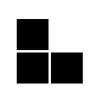
\includegraphics[scale=.50]{triomino}
   
\includegraphics[scale=.50]{triomino2}
  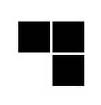
\includegraphics[scale=.50]{triomino3}
   
\includegraphics[scale=.50]{triomino4}
\end{figure}





\end{document}  